% -*- TeX -*- -*- UK -*- -*- PPR -*-
\documentclass[%
pdf,
%ps,accumulate,
%nocolorBG,
colorBG, slideColor,
%slideBW,
%draft,
total,
%frames
%azure
%blends
%prettybox
serpaggi
%contemporain
%nuancegris
%troispoints
%lignesbleues
%darkblue
%alienglow
%autumn
%
]{prosper}


%---------Packages-------------------------------------------------------

%\usepackage{prosper} % Just to make documentation easier to find
%\usepackage{seminar} % Just to make documentation easier to find
%\usepackage{xcolor}
\usepackage[centertags]{amsmath}
\usepackage{amssymb}
\usepackage{graphicx}
\usepackage{pstricks,pst-node,pst-text,pst-3d}
\usepackage{pstricks-add}

%---------Commands-------------------------------------------------------

\input{mydefs}
%\newcommand{\vp}{\vspace{0.5cm}}
\renewcommand{\slidebottommargin}{0.5in}
\renewcommand{\slidetopmargin}{0.8in}
\renewcommand{\paperwidth}{210mm}
\newcommand{\half}{\frac{1}{2}}
\newcommand{\CO}{\mathcal{O}}
\newcommand{\CL}{\mathcal{L}}
\newcommand{\CN}{\mathcal{N}}
\newcommand{\CM}{\mathcal{M}}
\newcommand{\CH}{\mathcal{H}}
\newcommand{\p}{\partial}
\newcommand{\apm}{{\alpha^{\prime}}}
\newcommand{\adg}{{a^{\dagger}}}
%\newcommand{\ra}{\rightarrow}
%\newcommand{\lr}{\leftrightarrow}
\newcommand{\ad}{{\dot{\alpha}}}
\newcommand{\bd}{{\dot{\beta}}}
\newcommand{\gd}{{\dot{\gamma}}}
\newcommand{\dd}{{\dot{\delta}}}
\newcommand{\ed}{{\dot{\epsilon}}}
\newcommand{\fb}{{\bar \phi}}
\newcommand{\Jb}{{\bar J}}
\newcommand{\Qb}{{\overline Q}}
\newcommand{\Sb}{{\overline S}}
\newcommand{\zb}{{\bar z}}
\newcommand{\wb}{{\overline w}}
\newcommand{\cb}{{\bar c}}
\newcommand{\ab}{{\bar a}}
\newcommand{\bb}{{\bar b}}
\newcommand{\bp}{{\bar\partial}}
\newcommand{\CP}{\mathbb{CP}}
\newcommand{\C}{\mathbb{C}}
\newcommand{\Z}{\mathbb{Z}}
\newcommand{\bR}{\mathbb{R}}
\newcommand{\tC}{\widetilde{C}}
\newcommand{\omwz}{\omega_\mathrm{WZ}}
\newcommand{\ombi}{\omega_\mathrm{BI}}
\newcommand{\thbi}{\theta_\mathrm{BI}}
\newcommand{\omfs}{\omega_\mathrm{FS}}
\newcommand{\omfl}{\omega_\mathrm{full}}
\newcommand{\svn}{_{\vec{n}}}

%---------Colours---------------------------------------------------------

%\newrgbcolor{LemonChiffon}{1. 0.98 0.8}
% \newrgbcolor{myellow}{.9 .8 .1}
% \newrgbcolor{myblue}{.2 .36 .77}
% \newrgbcolor{orange}{0.8 0.7 0.2}
% \newrgbcolor{myred}{0.95 0.0 0.0}

%---------Title-----------------------------------------------------------

\title {Giant gravitons and the supersymmetric states of  $\mathcal{N}=4$
Yang-Mills}
%
%\subtitle{based on \texttt{hep-th/0606087} with Indranil Biswas,
%Davide Gaiotto and Shiraz Minwalla}
%
\author{Subhaneil Lahiri}
%
\institution{%
Department of Physics, \\
Harvard University \\[0.5cm]
based on \texttt{hep-th/0606087} with Indranil Biswas, Davide
Gaiotto and Shiraz Minwalla}
%
%\slideCaption{Giant gravitons and SUSY states}

%---------Beginning--------------------------------------------------------

\begin{document}
\maketitle

%-------------Slide--------------------------------------------------------

%\overlays{}{
\begin{slide}{Outline}
%
 \begin{itemize}
    \item Gauge theories and gravity
    \item Black holes and supersymmetric states
    \item Giant gravitons
    \item Quantisation
    \item Conclusions and future directions
 \end{itemize}
%
\end{slide}
%}

%-------------Slide--------------------------------------------------------

\begin{slide}{Gauge theories and gravity}
%
 If we take the 't Hooft limit of a U(N) gauge theory ($N\ra\infty$,
 $\lambda=g^2N$ fixed) the $\frac{1}{N}$ expansion looks like
 perturbative string theory.

 \vp If we draw propagators and vertices for matrix fields as:
 %
 \begin{center}
    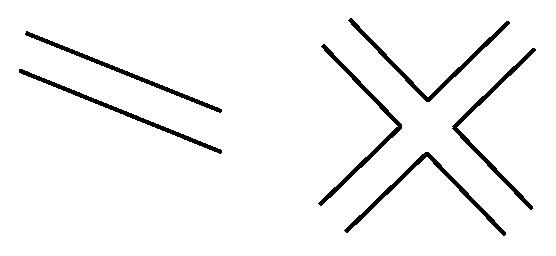
\includegraphics[width=3cm]{thooft.eps}
 \end{center}
 %
 Feynman diagrams look like two dimensional surfaces.
 %
 \begin{center}
    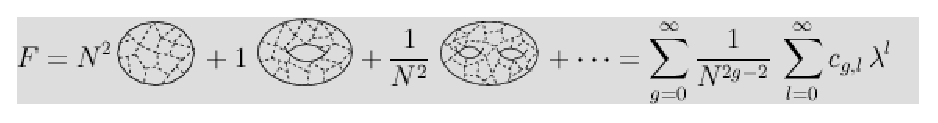
\includegraphics[width=10cm]{riem.eps}
 \end{center}
%
\end{slide}

%-------------Slide--------------------------------------------------------

%\overlays{}{
\begin{slide}{Gauge theories and gravity}
%
  The power of $\frac{1}{N}$ is ($2\times \#\, holes - 2$).

  \vp Just like $g_s$ in string theory:
   %
 \begin{center}
    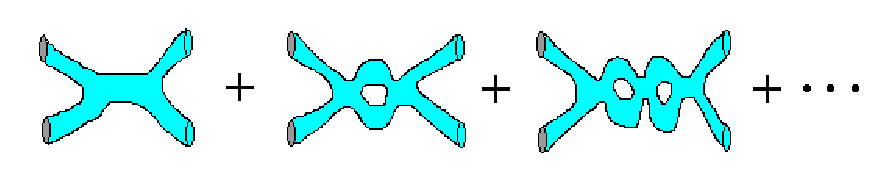
\includegraphics[width=10cm]{pert.eps}
 \end{center}
%
\end{slide}
%}

%-------------Slide--------------------------------------------------------

\overlays{2}{
\begin{slide}{The AdS/CFT correspondence}
%
 The best known case is a correspondence between:
 \begin{itemstep}
   \item U(N), $\CN=4$ super Yang-Mills on $S^3\times$ Time;
   \item Type IIB string theory on $AdS_5 \times S^5$ with $N$ units
   of five form flux;
 \end{itemstep}
 %
 \begin{center}
    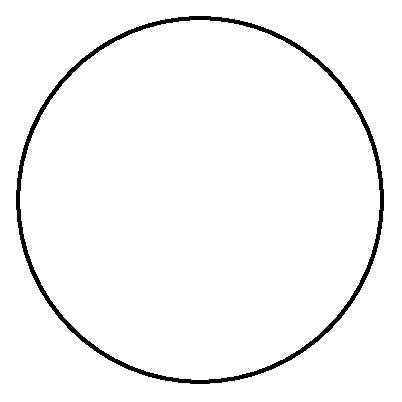
\includegraphics[width=2cm]{s3.eps}
    \fromSlide{2}{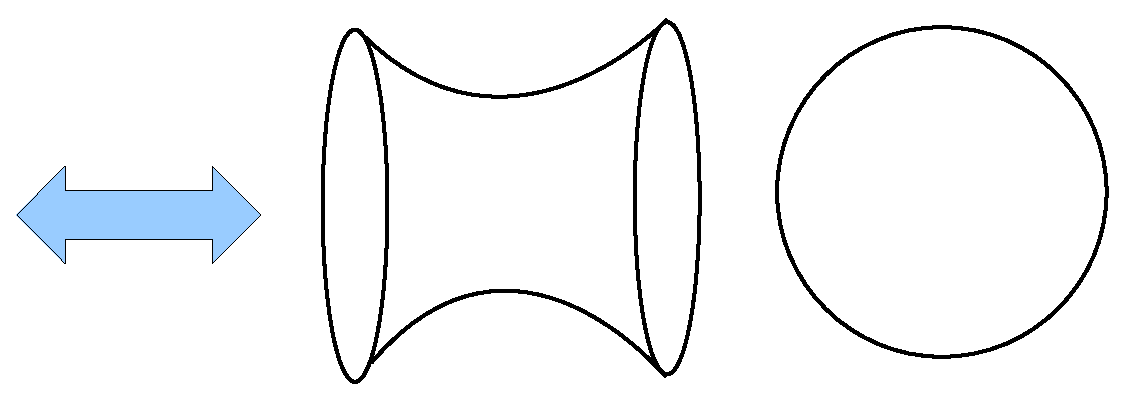
\includegraphics[width=6cm]{ads.eps}}
 \end{center}
%
\end{slide}
}

%-------------Slide--------------------------------------------------------

\overlays{2}{
\begin{slide}{Conformal invariance}
%
 $\CN=4$ super Yang-Mills theories happen to be scale invariant
 quantum mechanically as well as classically.

 \vp Scale invariant theories are usually invariant under conformal
 transformations: transformations that leave angles unchanged.

 \vp This group is SO(4,2).

 \FromSlide{2}\vp It is convenient to study conformal theories on
 $S^3$ rather than $\bR^3$ as there is a 1-1 correspondence between:
 {\darkred States on $S^3$} and {\darkred Local operators in
 $\bR^4$}.
%
\end{slide}
}

%-------------Slide--------------------------------------------------------

%\overlays{}{
\begin{slide}{Anti-de-Sitter space}
%
 Anti-de-Sitter space can be constructed as a hyperboloid in
 $\bR^{4,2}$:
 %
 \begin{equation*}
    -(x^{-1})^2 - (x^0)^2 + (x^1)^2 + (x^2)^2 + (x^3)^2 + (x^4)^2 =
    -R^2
 \end{equation*}

 It has the metric:
 %
 \begin{equation*}
    \dr s^2 = R^2(-\cosh^2\!\rho\, \dr t^2 + \dr\rho^2
    + \sinh^2\!\rho\, \dr\Omega^2)
 \end{equation*}
 %
 This has the symmetry group SO(4,2)

 \vp The boundary is conformally $S^3\times$Time.
%
\end{slide}
%}

%-------------Slide--------------------------------------------------------

\overlays{2}{
\begin{slide}{Super and R symmetries}
%
 The $\CN=4$ theory has 16 supersymmetries, $Q^i_\alpha$ and
 $\Qb_{i\,\ad}$, and their complex conjugates -- the superconformal
 symmetries $S_{i\,\alpha}$ and $\Sb^i_\ad$.

 \vp Correspondingly, IIB in $AdS_5\times S^5$ has 32 killing
 spinors.

 \FromSlide{2}\vp The $\CN=4$ theory also has an SU(4)=SO(6)
 R-symmetry that mixes the supersymmetries.

 \vp This is also the rotation group of $S^5$.
%
\end{slide}
}

%-------------Slide--------------------------------------------------------

%\overlays{}{
\begin{slide}{Counting states}
%
 We would like to classify the states of the theory using these
 symmetries.

 \vp i.e.\ count the number of states for each value of the Noether
 charges.

 \vp This can be summarised in a partition function:
 \begin{equation*}
    Z = \Tr\,\e^{\mu_i Q_i}
 \end{equation*}

%
\end{slide}
%}

%-------------Slide--------------------------------------------------------

%\overlays{}{
\begin{slide}{Parameter matching}
%
 The parameters are related by:
 %
 \begin{equation*}
   \begin{split}
     g_s & = \frac{\lambda}{N} \\
     \frac{R^4}{(\apm)^2}  & = 4\pi \lambda
   \end{split}
 \end{equation*}
 %
 This means:\\{\darkred
 \begin{center}
 \begin{tabular}{rcl}
 Low curvature &$\rightleftharpoons$& Strong coupling \\
 High curvature &$\rightleftharpoons$& Weak coupling
 \end{tabular}
 \end{center}}
%
\end{slide}
%}

%-------------Slide--------------------------------------------------------

%\overlays{}{
\begin{slide}{AdS-Schwarzschild black hole}
%
 The ``deconfinement'' phase transition in the gauge theory is dual
 to the formation of a black hole in the bulk.

 \vp Qualitative matching, but not quantitative -- the entropy is
 off by $\frac{3}{4}$.

 \vp The spectrum of the theory varies with $\lambda$.
 %
 \begin{center}
    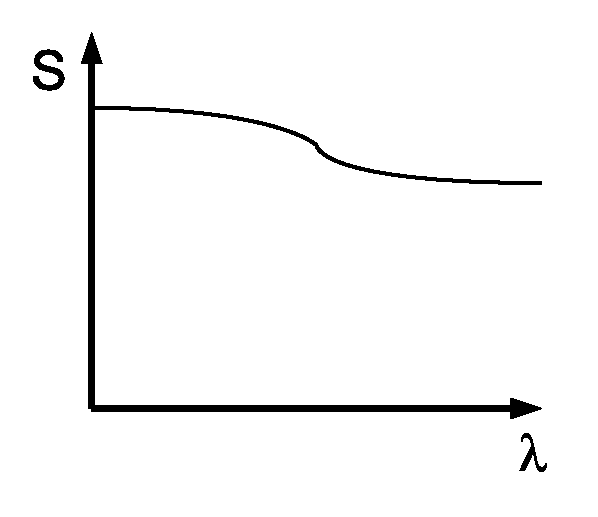
\includegraphics[width=4cm]{bhent.eps}
 \end{center}
%
\end{slide}
%}

%-------------Slide--------------------------------------------------------

\overlays{2}{
\begin{slide}{Supersymmetric spectrum}
%
 Supersymmetric states lie in short representations
 %
 \begin{center}
    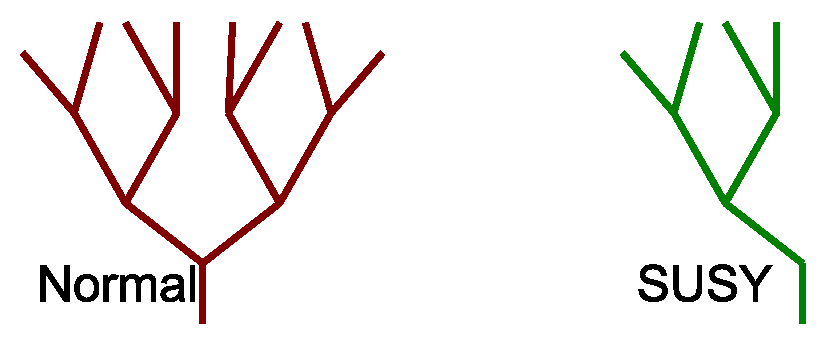
\includegraphics[height=2cm]{rep.eps}
 \end{center}
 %
 \FromSlide{2}SUSY $\ra$ non-SUSY requires short reps joining to
 form a long rep.
 %
 \begin{center}
    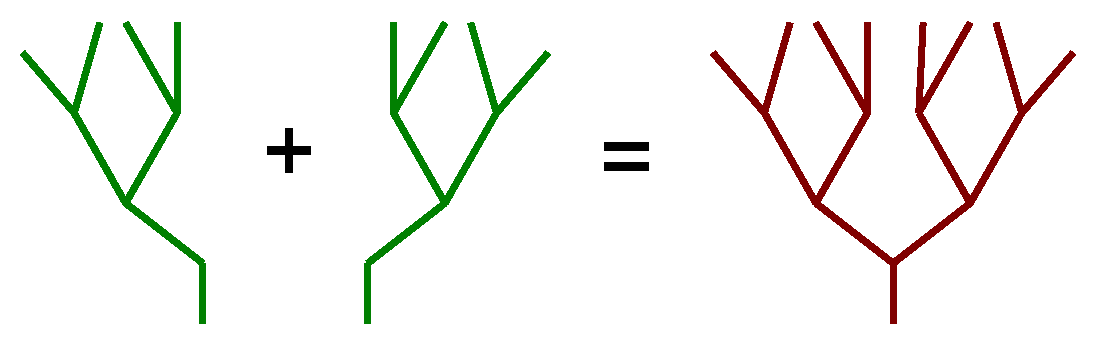
\includegraphics[height=2cm]{join.eps}
 \end{center}
 %
%
\end{slide}
}

%-------------Slide--------------------------------------------------------

\overlays{2}{
\begin{slide}{AdS$_5$ black holes}
%
  A general black hole has six parameters
  $(\Delta,J,\Jb,R_1,R_2,R_3)$.

  \vp For each value of $(J,\Jb,R_1,R_2,R_3)$, there is
  an extremal black hole.

  \FromSlide{2}\vp If these five charges satisfy an additional
  relation, this black hole preserves 1/16 of the supersymmetries.
  %
 \begin{center}
    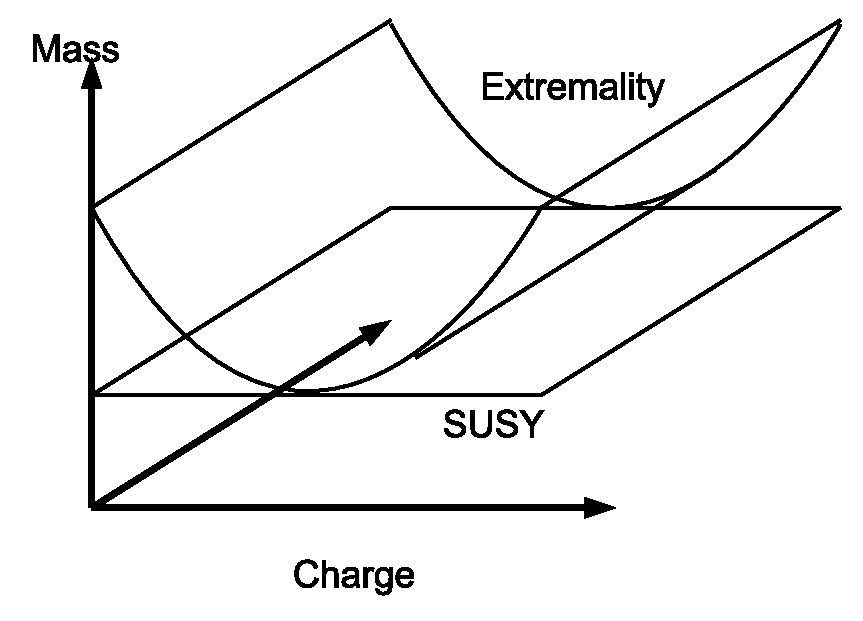
\includegraphics[width=4cm]{bh.eps}
 \end{center}
%
\end{slide}
}

%-------------Slide--------------------------------------------------------

\overlays{2}{
\begin{slide}{1/16 BPS states}
%
 At zero coupling:
 %
 \begin{itemize}
   \item Qualitative but not quantitative matching
   \item No sign of relation between charges
 \end{itemize}
 %
 \FromSlide{2}\vp At weak coupling:
 %
 \begin{itemize}
   \item Haven't found the spectrum
   \item Computing an index doesn't work
 \end{itemize}
%
\end{slide}
}

%-------------Slide--------------------------------------------------------

%\overlays{}{
\begin{slide}{1/8 BPS states}
%
 These are invariant under both components of $Q^1_\alpha$ and their
 complex conjugates $S_{1\,\alpha}$.

 \vp They are in 1-1 correspondence with cohomology classes of
 $Q^1_\alpha$, i.e.
 %
 \begin{equation*}
    \begin{split}
      Q \ket{\psi} & = 0 \\
      \ket{\psi} & \sim \ket{\psi} + Q \ket{\phi}
    \end{split}
 \end{equation*}
 %
 Each cohomology class contains one state that is also annihilated
 by $S$.
%
\end{slide}
%}

%-------------Slide--------------------------------------------------------

%\overlays{}{
\begin{slide}{1/8 BPS states}
%
 The supercharge acts (in $\CN=1$ language) as:
 %
 \begin{equation*}
 \begin{aligned}
  &Q_\alpha {\bar \phi}^m= 0\,,&
  %
  &Q_\alpha \phi_m = \psi_{m\alpha}\,, \\
  %
  &Q_\alpha \psi_{m \beta} =
        {\darkred g}\epsilon_{\alpha \beta} \epsilon_{mkl}
        [{\bar \phi}^{k}, {\bar \phi}^l ] \,,&
  %
  &Q_\alpha \lambda_{\beta}=
  f_{\alpha \beta} + {\darkred g}\epsilon_{\alpha \beta}
  [\phi_m, \bar{\phi}^m]\,, \\
  %
  &Q_\alpha  \bar{\psi}^{m}_{\dot \beta}
            = D_{\alpha {\dot \beta}} \bar{\phi}^{m}\,, &
  %
  &Q_\alpha  \bar{\lambda}_{\dot \beta} = 0\,,\\
  %
  &Q_\alpha A_{\beta {\dot \gamma}}
            = \epsilon_{\alpha \beta} \bar{\lambda}_{\dot \gamma}\,.&
  %
  \implies &Q_\alpha D_{\beta {\dot \gamma}}
            = {\darkred g}\epsilon_{\alpha \beta}
            [\bar{\lambda}_{\dot \gamma},\;\;]\,.&
 \end{aligned}
 \end{equation*}
 %
 The $Q$-closed letters are $\fb^m$ and $\bar{\lambda}_{\dot
 \beta}$. Their commutators are $Q$-exact. They are simultaneously
 diagonalisable in cohomology.

 \vp They can be counted in terms of eigenvalues.
%
\end{slide}
%}

%-------------Slide--------------------------------------------------------

\overlays{2}{
\begin{slide}{1/8 BPS states}
%
 The states built out of the scalars can be thought of as $N$ bosons
 moving in a three dimensional harmonic oscillator.

 \vp $(\fb^1_a)^{n_1}(\fb^2_a)^{n_2}(\fb^3_a)^{n_3}$
 maps onto boson number $a$ in the state $\ket{n_1,n_2,n_3}$.

 \vp Bosons because permutations are part of the gauge
 invariance.

 \FromSlide{2}\vp SO(6) charges are the total excitation $\#$'s of
 each oscillator.

 \vp Energies $<<N$ described by multi-gravitons.

 Energies $\sim N$ described by giant gravitons.
%
\end{slide}
}

%-------------Slide--------------------------------------------------------

\overlays{5}{
\begin{slide}{Giant gravitons}
%
 {\darkred Dubious analogy:} neutral particle moving in a magnetic field.
 %
 \begin{center}
  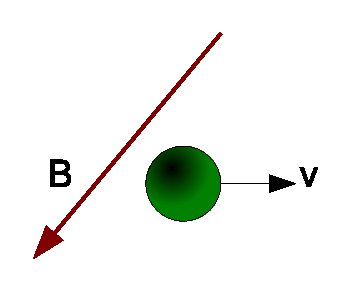
\includegraphics[height=1.5cm]{analogy1.eps}
  \fromSlide{2}{\hspace{1cm}
  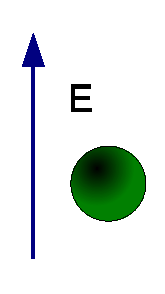
\includegraphics[height=1.5cm]{analogy2.eps}}
  \fromSlide{3}{\hspace{1cm}
  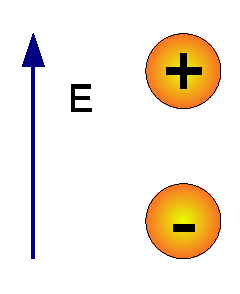
\includegraphics[height=1.5cm]{analogy3.eps}}
 \end{center}
 %
 \FromSlide{4}Graviton moving fast around $S^5$
 %
 \begin{center}
  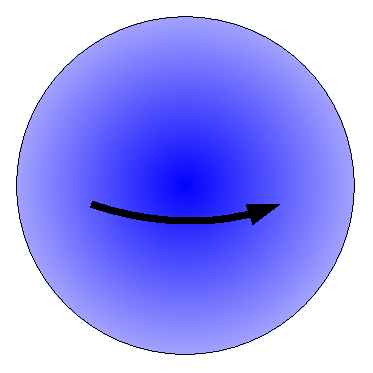
\includegraphics[height=2cm]{grav.eps}%\hspace{1cm}
  \fromSlide{5}{
  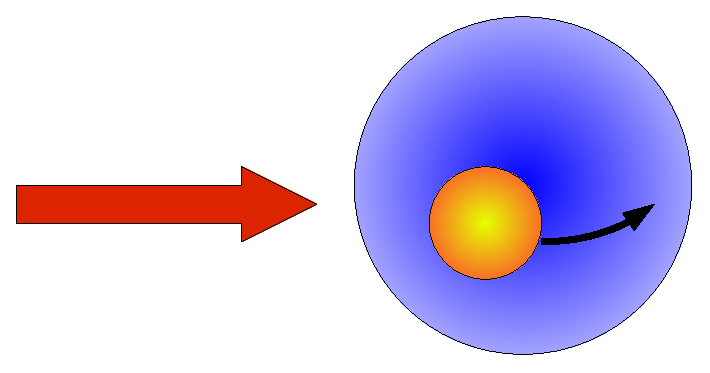
\includegraphics[height=2cm]{giant.eps}}
 \end{center}
 %
 \FromSlide{5} Likes to puff out into a D3 brane.

 \vp Quantising these produces finite $N$, 1/2 BPS spectrum.
%
\end{slide}
}

%-------------Slide--------------------------------------------------------

\overlays{4}{
\begin{slide}{1/8 BPS giant gravitons}
%
 Mikhailov's construction:
 %
 \begin{itemstep}
   \item Embed $S^5$ in $\C^3$
   %
   \begin{equation*}
    |x|^2+|y|^2+|z|^2=1
   \end{equation*}

   \item Pick a holomorphic function $f(x,y,z)$

   \item The D3-brane wraps the intersection of the surface $f(\e^{-\ir t}x,
   \e^{-\ir t}y, \e^{-\ir t}z) = 0$ with the $S^5$.
 \end{itemstep}

 \FromSlide{4}\vp It can be shown that this preserves 1/8 of the
 supersymmetries.

 \vp Doesn't include worldvolume gauge fields and fermions.
%
\end{slide}
}

%-------------Slide--------------------------------------------------------

\overlays{3}{
\begin{slide}{Quantisation}
%
 First we need to describe the system in the Hamiltonian formalism.

 \FromSlide{2}\vp We need a phase space and a Poisson bracket:
 %
 \begin{equation*}
    \{ x^i , x^j \} = \omega^{ij}\,, \qquad
    \{ f , g \} = \omega^{ij} (\p_i f) (\p_j g)\,,
 \end{equation*}
 %
 or, equivalently, a symplectic form: $\omega_{ij} =
 \brk{\omega^{ij}}^{-1}$.

 \FromSlide{3}\vp This must be closed and non-degenerate:
 %
 \begin{equation*}
    \dr\omega=0\,, \qquad \det\omega \neq 0\,.
 \end{equation*}

 Then we can use the standard procedure of Geometric Quantisation.
%
\end{slide}
}

%-------------Slide--------------------------------------------------------

\overlays{2}{
\begin{slide}{Crnkovic-Witten-Zuckerman formalism}
%
 We can identify the phase space with the space of solutions to the
 equations of motion.

 \FromSlide{2}\vp We then find $\omega$ by plugging the solutions
 into:
 %
 \begin{equation*}
    \omega = \int\!\dr x\: \delta p_i \wedge \delta \phi^i
 \end{equation*}
 %
 where $\phi^i$ are the dynamical fields and $p_i$ are their
 conjugate momenta:
 %
 \begin{equation*}
    p_i = \pdiff{L}{\dot{\phi}^i\mbox{}}
 \end{equation*}
%
\end{slide}
}

%-------------Slide--------------------------------------------------------

\overlays{2}{
\begin{slide}{Symplectic form}
%
 Using the Born-Infeld + Wess-Zumino action:
 %
 \begin{equation*}
  \begin{split}
   S&= S_\mathrm{BI}+S_\mathrm{WZ} \\
    &=\frac{1}{(2 \pi)^3 (\apm)^2 g_s}
    \int\!\!\dr^4\sigma\, \sqrt{-\tilde{g}}  +
    \int\!\!\dr t\,\dr^3\sigma\:
     A_{\mu_0\mu_1\mu_2\mu_3}\, \dot{x}^{\mu_0}\,
       \frac{\p x^{\mu_1}}{\p\sigma^1}
       \frac{\p x^{\mu_2}}{\p\sigma^2}
       \frac{\p x^{\mu_3}}{\p\sigma^3}\, ,
  \end{split}
 \end{equation*}
 %
 \FromSlide{2}we can find the symplectic form:
 %
 \begin{multline*}
  \omfl = \ombi +\omwz =
  \frac{N}{2\pi^2} \int_\Sigma\!\! \dr^3 \sigma\:
   \delta\! \left( \sqrt{-g} g^{0\alpha}
   \frac{\partial x^\mu}{\partial \sigma^\alpha}
   {G}_{\mu \nu}\right) \wedge \delta x^\nu\\
  +\frac{2N}{\pi^2}\int_\Sigma\!\!\dr^3\sigma\:
    \frac{\delta x^{\lambda}\wedge \delta x^{\mu}}{2} \left(
     \frac{\p x^{\nu}}{\p\sigma^1}
     \frac{\p x^{\rho}}{\p\sigma^2}
     \frac{\p x^{\sigma}}{\p\sigma^3}\right)
    \epsilon_{\lambda\mu\nu\rho\sigma}\, .
 \end{multline*}
%
\end{slide}
}

%-------------Slide--------------------------------------------------------

\overlays{2}{
\begin{slide}{Mikhailov's phase space}
%
 Solutions parameterised by one holomorphic function.

 \vp This is an infinite dimensional space. We regulate it by
 restricting to polynomials made from a finite number of monomials:
 %
 \begin{equation*}
    f(z_1,z_2,z_3) = \sum_{\vec{n} \in C} c\svn\,
       (z^1)^{n_1} (z^2)^{n_2} (z^3)^{n_3}\,.
 \end{equation*}
 %
 \FromSlide{2}$c\svn$ and $\lambda c\svn$ describe the same surface.

 \vp {\darkred It looks like $\CP^{n_C-1}$.}
%
\end{slide}
}

\begin{slide}{But unfortunately \ldots}
%
 \ldots not all surfaces touch the sphere:
 %
 \begin{center}
    \includegraphics[width=10cm]{touch.eps}
 \end{center}
 %
 \vp Eats holes out of phase space.
%
\end{slide}

%-------------Slide--------------------------------------------------------

\overlays{2}{
\begin{slide}{Geometric quantisation of $\CP^n$}
%
 $\CP^n$ has a canonical two-form (Fubini-Study):
 %
 \begin{equation*}
    \omfs = \frac{1}{4\pi\ir}\frac{1}{|z|^2}
    \brk{\dr\zb^i-\frac{\zb^iz^j}{|z|^2}\dr\zb^j}\wedge
    \brk{\dr z^i - \frac{z^i\zb^j}{|z|^2}\dr z^j}\,.
 \end{equation*}
 %
 Suppose that our symplectic form is in the cohomology class $(2\pi
 N)[\omfs]$.

 \FromSlide{2}\vp It is a standard result that the Hilbert space is the
 space of {\darkred degree $N$ homogeneous polynomials} in the $z^i$.
%
\end{slide}
}

%-------------Slide--------------------------------------------------------

\overlays{3}{
\begin{slide}{3D harmonic oscillator}
%
 We can map this to the 3D harmonic oscillator as follows:

 \vp $c\svn \ra a\svn^\dagger$ : the creation operator for a
 particle in the state $\ket{n_1,n_2,n_3}$.

 \FromSlide{2}\vp A monomial of degree $N$ acting on the vacuum
 produces a $N$-particle state.

 \FromSlide{3}\vp These states transform the same way under U(3) as
 our 3D harmonic oscillator.
%
\end{slide}
}

%-------------Slide--------------------------------------------------------

\overlays{4}{
\begin{slide}{Problems}
%
 \begin{itemstep}
 %
  \item Some surfaces do not touch the sphere, e.g.
  %
  \begin{equation*}
    c_i z^i - 1 = 0 \quad \text{for} \quad |c|^2<1\,.
  \end{equation*}
  %
  \item Singularities when the function factorises - the surface
  degenerates, e.g.
  %
  \begin{equation*}
    x^2 + y^2 + \epsilon z^2 = 0 \quad \text{as} \quad \epsilon\ra
    0\,.
  \end{equation*}
  %
  \item Factorised functions where one factor doesn't touch the
  sphere.
  %
  \item Finding the cohomology class of $\omega$.
  %
 \end{itemstep}
%
\end{slide}
}

%-------------Slide--------------------------------------------------------

\begin{slide}{Example: Linear functions}
%
 Let's look at the space of functions $f(z^i) = c_i z^i -1$.

 \vp The symplectic form is:
 %
 \begin{equation*}
   \omega =2N\left[
   \left(\frac{1}{|c|^2}-\frac{1}{|c|^4}\right)
      \frac{\dr\cb^i\wedge\dr c_i}{ 2\ir}
   -\left(\frac{1}{|c|^2}-\frac{2}{|c|^4}\right)
      \frac{\cb^ic_j}{|c|^2}\frac{\dr\cb^j\wedge\dr c_i}{ 2\ir}
   \right].
 \end{equation*}

 It is zero inside $|c|^2<1$ and has four null directions on the
 boundary.

 \vp While it is not zero at the boundary, its restriction to the
 boundary is.
%
\end{slide}

%-------------Slide--------------------------------------------------------

\overlays{2}{
\begin{slide}{Contracting the hole}
%
 Coordinate change:
 %
 \begin{equation*}
    w_i = c_i \, \sqrt{\frac{|c|^2-1}{|c|^2}}
 \end{equation*}
 %
 Shrinks sphere $|c|^2=1$ to the point $|w|^2=0$. \FromSlide{2}We get:
 %
 \begin{equation*}
  \omega = \frac{2N}{1+|w|^2} \left(
        \frac{\dr\wb^i \wedge \dr w_i}{2\ir}
        -\frac{w_i \wb^j}{1+|w|^2}
              \frac{\dr\wb^i \wedge \dr w_j}{2\ir}
        \right)
 \end{equation*}
 %
 {\darkred This is precisely $(2\pi N)\omfs$ on $\CP^3$ !}
%
\end{slide}
}

%-------------Slide--------------------------------------------------------

\overlays{3}{
\begin{slide}{General case}
%
 Define the distance function: $\rho(c,\cb)$ - the minimum distance
 from the origin of $\C^3$ to the surface.

 \vp The boundary of the hole is $\rho=1$

 \FromSlide{2}\vp Under $c\svn \ra \lambda^{-(n_1+n_2+n_3)} c\svn$,
 we have $\rho \ra \lambda\rho$.

 \vp Each ray $c\svn(\lambda) = \lambda^{-(n_1+n_2+n_3)}
 c\svn^{(0)}$ intersects the boundary $\rho=1$ once.

 \FromSlide{3}\vp This means that the hole has the topology of a
 ball -- can be contracted, e.g.\ with $\lambda=(1-\rho^2)^{-1/2}$.
%
\end{slide}
}

%-------------Slide--------------------------------------------------------

\overlays{2}{
\begin{slide}{Factorised submanifolds}
%
 There are submanifolds of phase space where the function
 factorises.

 \vp These submanifolds also have holes. These holes, and their
 intersections with each other, are also balls.

 \FromSlide{2}\vp This means we can contract all of the holes
 without changing the topology.

 \vp {\darkred The phase space is $\CP^{n_C-1}$ after all!}

 \vp As $\rho$ is U(3) invariant, this doesn't change the charges of
 the coordinates.
%
\end{slide}
}

%-------------Slide--------------------------------------------------------

\begin{slide}{Geometric description of $\omega$}
%
 \textbf{\darkred Wess-Zumino contribution:}

 \begin{equation*}
  \omwz = \frac{2N}{\pi^2}\int_\Sigma\!\!\dr^3\sigma\:
    \frac{\delta x^{\lambda}\wedge \delta x^{\mu}}{2} \left(
     \frac{\p x^{\nu}}{\p\sigma^1}
     \frac{\p x^{\rho}}{\p\sigma^2}
     \frac{\p x^{\sigma}}{\p\sigma^3}\right)
    \epsilon_{\lambda\mu\nu\rho\sigma}\, .
 \end{equation*}
 %
 For two deformations of the surface, this is $\frac{2N}{\pi^2}$
 times the volume swept out.
%
\end{slide}

%-------------Slide--------------------------------------------------------

\begin{slide}{Geometric description of $\omega$}
%
 \textbf{\darkred Born-Infeld contribution:}

 \vp For Mikhailov's solutions, we can write:
 %
 \begin{equation*}
 \begin{split}
   \ombi & = \dr\thbi \\
   \thbi & = \frac{N}{\pi^2}
     \int_S\!\!\dr^4\sigma\:
        \epsilon_{\mu_1\cdots\mu_6}
        \left[
        \frac{\p x^{\mu_1}}{\p\sigma^1}
        \cdots
        \frac{\p x^{\mu_4}}{\p\sigma^4}
        \right]
        e_\perp^{\mu_5}\,\delta x^{\mu_6}
        \,\delta\!\left(|z^i|^2-1\right)\,,
 \end{split}
 \end{equation*}
 %
 i.e. compute $\frac{N}{2\pi^2}$ times the volume, inside a ball of
 radius $r$, swept out by a deformation of $S$ and the unit radial
 vector $e_\perp$. Differentiate it with respect to $r$ and set
 $r=1$.
%
\end{slide}

%-------------Slide--------------------------------------------------------

\overlays{3}{
\begin{slide}{Singularities of $\omega$}
%
 These can be formally rewritten as fibre integrals of closed forms.

 \vp This means $\omega$ is a current -- i.e. $\int\beta\wedge\omega$
 is finite, even if $\omega$ isn't.

 \FromSlide{2}\vp We can also see that $\omega$ vanishes when
 restricted to the boundary, {\darkred so no singularities from
 contracting it.}

 \FromSlide{3}\vp {\darkred This is enough for geometric quantisation}
%
\end{slide}
}

%-------------Slide--------------------------------------------------------

\overlays{2}{
\begin{slide}{Cohomology class of $\omega$}
%
 Every closed two form in $\CP^{n_C-1}$ can be written as:
 %
 \begin{equation*}
    M\omfs+\dr\beta\,.
 \end{equation*}
 %
 We want to determine $M$.

 \FromSlide{2}\vp Consider two sets of monomials $\tC \subset C$.
 Restricting the the phase space from $C$ to $\tC$ maps:
 %
 \begin{equation*}
  \begin{split}
    \CP^{n_C-1} & \ra \CP^{n_{\tC}-1}\,, \\
    \omfs  & \ra \omfs\,.
  \end{split}
 \end{equation*}
 %
 This means $M_C=M_{\tC}$
%
\end{slide}
}

%-------------Slide--------------------------------------------------------

\overlays{5}{
\begin{slide}{Cohomology class of $\omega$}
%
 Looking at a tree like:
 %
 \begin{equation*}
    \setlength{\arraycolsep}{0.5cm}
    \begin{array}{ccc}
       & \rnode{a}{}C_1 \cup C_2 \rnode{b}{} & \\[1.0cm]
       \rnode{c}{} & & \rnode{d}{}\\[-0.3cm]
       C_1 & & C_2
    \end{array}
    \psset{nodesep=5pt,arrows=->}
    \ncline[linecolor=darkblue]{a}{c}
    \fromSlide*{2}{
    \Bput{\darkred M_{C_1 \cup C_2}=M_{C_1}}}
    \ncline[linecolor=darkblue]{b}{d}
    \fromSlide*{3}{
    \Aput{\darkred M_{C_1 \cup C_2}=M_{C_2}}}
 \end{equation*}
 %
 \FromSlide{4}We see that $M_{C_1}=M_{C_2}$.

 \FromSlide{5}\vp We have already found $M$ for linear functions, so
 {\darkred $M=2\pi N$ for all $C$.}
%
\end{slide}
}


%-------------Slide--------------------------------------------------------

\overlays{5}{
\begin{slide}{Summary}
%
  \begin{itemstep}
    \item The Phase space is $\CP^{n_C-1}$
    \item The symplectic form is cohomologically $(2\pi N)\omfs$
    \item The coordinates have U(3) charges $(n_1,n_2,n_3)$
    \item This is isomorphic to the 3D harmonic oscillator
  \end{itemstep}
  %
  \FromSlide{5} This gives the partition function
  \begin{equation*}
    \sum_N \zeta^N Z_N(\mu_1,\mu_2,\mu_3) =
      \prod\svn\frac{1}{1-\zeta\e^{-\mu_i n_i}}
  \end{equation*}
%
\end{slide}
}

%-------------Slide--------------------------------------------------------

\overlays{6}{
\begin{slide}{Conclusions and future directions}
%
  We get exact (finite $N$) matching between the gauge theory and
  giant gravitons.

  \FromSlide{2}\vp We are getting ordinary gravitons by quantising
  D-branes.

  \FromSlide{3}\vp Giant/goliath duality still works.

  \FromSlide{4}\vp Should be extended to include worldvolume gauge
  fields and fermions.

  \FromSlide{5}\vp Can be extended to other AdS/CFT duals.

  \FromSlide{6}\vp Classical 1/16 BPS giants are known, but much
  harder to quantise.
%
\end{slide}
}

%-------------Slide--------------------------------------------------------

\overlays{2}{
\begin{slide}{Dual giants}
%
  These are spherically symmetric in $AdS_5$, point-like in $S^5$
  and move as: $(x,y,z)=(x_0\e^{\ir t},y_0\e^{\ir t},z_0\e^{\ir
  t})$.

  \vp The phase space is given by the radius of the giant and an
  initial position on $S^5$: $\bR^+\times S^5 = \C^3$.

  \FromSlide{2}\vp This has the standard symplectic form and Noether
  charges $\half N (x^2,y^2,z^2)$.

  \vp This \emph{\darkred is} the 3D harmonic oscillator.
%
\end{slide}
}

%-------------Slide--------------------------------------------------------

\overlays{4}{
\begin{slide}{1/16 BPS giants}
%
  As well as embedding $S^5$ in $\C^3$, we can embed $AdS_5$ in
  $\C^{2,1}$ as: $|w|^2-|u|^2-|v|^2=1$.

  \FromSlide{2}\vp Pick three holomorphic functions,
  $f_i(w_j,x_k)$ that satisfy a homogeneity condition
  %
  \begin{equation*}
  f_i\prn{\frac{w_j}{\lambda},\lambda x_k} =
  \lambda^n f_i(w_j,x_k)\,.
  \end{equation*}

  \FromSlide{3}\vp The worldvolume is given by the the intersection
  of the surface $f_i=0$ with $AdS_5 \times S^5$.

  \FromSlide{4}\vp This is much harder to quantise.
%
\end{slide}
}













%-End--------------------------------------------------------------------


\end{document}


%-End--------------------------------------------------------------------
%-----End----------------------------------------------------------------
%---------End------------------------------------------------------------
%-------------End--------------------------------------------------------



\begin{slide}{Geometric quantisation}
 Suppose we are given a classical phase space $\CM$ with a Poisson
 bracket:
 \begin{equation*}
    \{ x^i , x^j \} = \omega^{ij}\,, \qquad
    \{ f , g \} = \omega^{ij}\p_if\p_jg\,,
 \end{equation*}
 or, equivalently, a symplectic form: $\omega_{ij} =
 \brk{\omega^{ij}}^{-1}$.
\vp

 Locally, we can write $\omega_{ij}=\p_i\theta_j - \p_j\theta_i$,
 where $\theta$ is called the symplectic potential. Globally, we
 might have to use different $\theta$'s in different patches that
 are related by gauge transformations in the overlaps:
 $\theta^{(m)}_i = \theta^{(n)}_i + \p_iu^{(mn)}$.
\vp

 We would like to construct a corresponding quantum theory.
\end{slide}

%-------------Slide--------------------------------------------------------

\overlays{5}{
\begin{slide}{Geometric quantisation}
 That is, we want a Hilbert space $\CH$ and a map from classical
 observables (functions on $\CM$) to their quantum
 counterparts (operators on $\CH$) that:
 \begin{itemize}
   \FromSlide{2}\item is linear
   \FromSlide{3}\item maps real functions to hermitian operators
   \FromSlide{4}\item maps poisson brackets to commutators
   \FromSlide{5}\item maps one to the identity operator.
 \end{itemize}
\end{slide}}

%-------------Slide--------------------------------------------------------

\overlays{3}{
\begin{slide}{First guess}
 $\CH$ consists of normalisable functions on $\CM$ with the inner
 product:
 \begin{equation*}
    \braket{\phi}{\psi} = \int_\CM \frac{\omega^n}{(2\pi)^n n!}
     \; \bar{\phi}\psi\,.
 \end{equation*}
 The operators are: $\hat{A} = -\ir\hbar\omega^{ij}(\p_iA)\p_j$.

 \vp\FromSlide{2}This has the property: $[\hat{A},\hat{B}] = \ir\hbar
 \hat{C}$, where $\brc{A,B}=C$.

 \vp\FromSlide{3}{\red Problem:} $1\ra0$, so $\brk{\hat{x},\hat{p}}
 = 0$.
\end{slide}}

%-------------Slide--------------------------------------------------------

\overlays{3}{
\begin{slide}{Second guess}
 Try: $\hat{A} = -\ir\hbar\omega^{ij}(\p_iA)\p_j + A$.

 \vp\FromSlide{2}This has $1\ra\hat{1}$.

 \vp\FromSlide{3}{\red Problem:} $[\hat{A},\hat{B}] \neq \ir\hbar
 \hat{C}$.
\end{slide}}

%-------------Slide--------------------------------------------------------

\overlays{3}{
\begin{slide}{Solution}
 Replace $\p_i$ with the covariant derivative $D_i= \p_i -\frac{\ir}{\hbar}
 \theta_i$:
 \begin{equation*}
    \hat{A} = -\ir\hbar\omega^{ij}(D_iA)\p_j + A\,.
 \end{equation*}

 \vp\FromSlide{2}This has $[\hat{A},\hat{B}] = \ir\hbar \hat{C}$ and
 $1\ra\hat{1}$.

 \vp\FromSlide{3}{\red But:} The covariant derivative is only
 covariant when acting on charged fields.
\end{slide}}

%-------------Slide--------------------------------------------------------

\overlays{2}{
\begin{slide}{}
 This means that the wavefunctions have to transform under gauge
 transformations
 \begin{equation*}
    \theta_i \ra \theta_i + \p_i u \qquad
    \psi \ra \psi\e^{\ir u}\,.
 \end{equation*}

 \FromSlide{2}In particular:
 \begin{equation*}
    \psi^{(m)} = \psi^{(n)} \e^{\ir u^{(mn)}}\,.
 \end{equation*}

 \vp This can be summarised as: the wavefunctions are sections of a
 line bundle with curvature $\omega$
\end{slide}}

%-------------Slide--------------------------------------------------------

\begin{slide}{Geometric description of $\omega$}
%
 \textbf{\darkred Wess-Zumino contribution:}

 \begin{equation*}
  \omwz = \frac{2N}{\pi^2}\int_\Sigma\!\!\dr^3\sigma\:
    \frac{\delta x^{\lambda}\wedge \delta x^{\mu}}{2} \left(
     \frac{\p x^{\nu}}{\p\sigma^1}
     \frac{\p x^{\rho}}{\p\sigma^2}
     \frac{\p x^{\sigma}}{\p\sigma^3}\right)
    \epsilon_{\lambda\mu\nu\rho\sigma}\, .
 \end{equation*}
 %
 For two deformations of the surface, this is $\frac{2N}{\pi^2}$
 times the volume swept out.

 \vp This can be stated more formally:

 \vp Let $\CM$ be a subbundle of $\CP^{n_C-1}\times S^5$ consisting
 of $(x,z)$ s.t. $z$ lies in the surface given by $x$.
%
\end{slide}

%-------------Slide--------------------------------------------------------

\overlays{5}{
\begin{slide}{Geometric description of $\omega$}
%
 We can draw this as
 %
 \begin{equation*}
    \setlength{\arraycolsep}{1cm}
    \begin{array}{cc}
       \;\;\;\CM\;\;\rnode{a}{} & \rnode{b}{}\CP^{n_C-1}\times S^5\\[-0.2cm]
       \fromSlide{3}{{\red f^*(\epsilon_5)}} & \fromSlide{2}{{\red \epsilon_5}}\\[1.0cm]
       \phantom{\;\;\;\CM\;\;}\rnode{c}{} & \\[-0.3cm]
       \CP^{n_C-1} & \\[-0.3cm]
       \fromSlide{4}{{\red \omwz}} & \\
    \end{array}
    \psset{hooklength=3mm,hookwidth=-2mm}
    \psset{nodesep=5pt,arrows=H->}
    \ncline[linecolor=darkblue]{a}{b}\Aput{f}
    \psset{nodesep=5pt,arrows=->}
    \ncline[linecolor=darkblue]{a}{c}\Bput{g}
 \end{equation*}
 %
 \FromSlide{5}and we have $\omwz=
 \frac{2N}{\pi^2}\int_{\CM/\CP^{n_C-1}}f^*(\epsilon_5)$.

 \vp As the fibre integral of a closed form, it is a closed current.
%
\end{slide}
}

%-------------Slide--------------------------------------------------------

\overlays{3}{
\begin{slide}{Currents}
%
 A current is something that can be integrated against another form,
 i.e.
 %
 \begin{equation*}
    \int \beta \wedge \omega
 \end{equation*}
 %
 is well defined.

 \FromSlide{2}\vp We can see that $\omwz$ is a current by lifting the
 integral to $\CM$:
 %
 \begin{equation*}
    \int_{\CP^{n_C-1}} \beta \wedge \omega =
    \int_\CM g^*(\beta) \wedge f^*(\epsilon_5)
 \end{equation*}

 \FromSlide{3}\vp {\darkred This is enough for geometric
 quantisation.}
%
\end{slide}
}

%-------------Slide--------------------------------------------------------

\begin{slide}{Geometric description of $\omega$}
%
 \textbf{\darkred Born-Infeld contribution:}

 \vp For Mikhailov's solutions, we can write:
 %
 \begin{equation*}
 \begin{split}
   \ombi & = \dr\thbi \\
   \thbi & = \frac{N}{\pi^2}
     \int_S\!\!\dr^4\sigma\:
        \epsilon_{\mu_1\cdots\mu_6}
        \left[
        \frac{\p x^{\mu_1}}{\p\sigma^1}
        \cdots
        \frac{\p x^{\mu_4}}{\p\sigma^4}
        \right]
        e_\perp^{\mu_5}\,\delta x^{\mu_6}
        \,\delta\!\left(|z^i|^2-1\right)\,,
 \end{split}
 \end{equation*}
 %
 i.e. compute the volume, inside a ball of radius $r$,
 swept out by a deformation of $S$ and the unit radial vector
 $e_\perp$. Differentiate it with respect to $r$ and set $r=1$.

 \vp {\darkred This is also a current.}
%
\end{slide}

%-------------Slide--------------------------------------------------------

\overlays{7}{
\begin{slide}{$\omega$ at the boundaries}
%
 The boundaries are surfaces that just touch the sphere from the
 outside.

 \begin{tabular}{ll}
  \FromSlide{2}$x^2-1$         &
         \FromSlide{2}touches at two points.\\
  \FromSlide{3}$x^2+y^2-1$     &
         \FromSlide{3}touches on a circle.\\
  \FromSlide{4}$x^2+y^2+z^2-1$ &
         \FromSlide{4}touches on a two-sphere.
 \end{tabular}

 \FromSlide{5}\vp It can be shown that the touching is at most two
 dimensional, therefore $\omwz=0$ at the boundary

 \FromSlide{6}\vp $\thbi$ is also zero (as a current) at the
 boundary - take the derivative as the limit from below.

 \FromSlide{7}\vp {\darkred So we don't get singularities from
 contracting the boundary.}
%
\end{slide}
}
